\documentclass{beamer}
\usepackage[T1]{fontenc}
\usepackage[utf8]{inputenc}
\usepackage[cyr]{aeguill}
\usepackage[english]{babel}
\usepackage{amsmath,amssymb,amsthm}
\usepackage{bm}
\usepackage{graphicx}
\usepackage{geometry}
\usepackage{tikz}
\usepackage{diffcoeff}
\usepackage{tcolorbox}

\usepackage{comment}

\usepackage{natbib}
\usepackage{bibentry}


\usepackage{multirow}

\usepackage{xcolor,colortbl}

\newcommand{\mc}[2]{\multicolumn{#1}{c}{#2}}

\definecolor{Green}{rgb}{0.4,1,0.4}
\definecolor{Red}{rgb}{1,0.2,0.2}
\definecolor{Yellow}{rgb}{1,1,0.4}
\definecolor{Orange}{rgb}{0.8,0.4,0.2}
\definecolor{Blue}{rgb}{0.4,0.8,0.8}

\newcolumntype{n}{>{\columncolor{Red}}c}
\newcolumntype{g}{>{\columncolor{Green}}c}
\newcolumntype{m}{>{\columncolor{Yellow}}c}
\newcolumntype{b}{>{\columncolor{Orange}}c}
\newcolumntype{o}{>{\columncolor{Blue}}c}


\usepackage{movie15}
%\usepackage{multimedia}
%\usepackage{media9}

\graphicspath{{./Figures/}{./Animations/}}

\newcommand{\tens}[1]{%
	\mathbin{\mathop{\otimes}\displaylimits_{#1}}%
}

\newtheorem{remark}{Remark}
\newtheorem{proposition}{Proposition}

\makeatletter \renewcommand\d[1]{\ensuremath{%
		\;\mathrm{d}#1\@ifnextchar\d{\!}{}}}
\makeatother

\mode<presentation> {
	%\usetheme{Singapore}
	\usetheme{Madrid}
}
\usefonttheme{serif}
\usecolortheme{beaver}

\DeclareMathOperator*{\argmax}{arg\,max}
\DeclareMathOperator*{\argmin}{arg\,min}
\DeclareMathOperator{\Tr}{Tr}

\def\onedot{$\mathsurround0pt\ldotp$}
\def\cddot{% two dots stacked vertically
	\mathbin{\vcenter{\baselineskip.67ex
			\hbox{\onedot}\hbox{\onedot}}%
}}



\newcommand{\matr}[1]{\bm{#1}} 

\newcommand{\blue}[1]{\textcolor{blue}{#1}}
\newcommand{\red}[1]{\textcolor{red}{#1}}
\newcommand{\green}[1]{\textcolor{red}{#1}}

% make bibliography entries smaller
%\renewcommand\bibfont{\scriptsize}
% If you have more than one page of references, you want to tell beamer
% to put the continuation section label from the second slide onwards
%\setbeamertemplate{frametitle continuation}[from second]
% Now get rid of all the colours
%\setbeamercolor*{bibliography entry title}{fg=black}
%\setbeamercolor*{bibliography entry author}{fg=black}
%\setbeamercolor*{bibliography entry location}{fg=black}
%\setbeamercolor*{bibliography entry note}{fg=black}
% and kill the abominable icon
%\setbeamertemplate{bibliography item}{}


\expandafter\def\expandafter\insertshorttitle\expandafter{%
	\insertshorttitle\hfill%
	\insertframenumber\,/\,\inserttotalframenumber}

%
%\addtobeamertemplate{frametitle}{}{
%	\vskip-1em
%	\begin{tikzpicture}[remember picture,overlay]
%	\node[anchor=north east,yshift=-10pt] at (current page.north east) {
\includegraphics[height=0.8cm]{ISAE-SUPAERO.png}};
%	\end{tikzpicture}
%}

\title[INFIDHEM Workshop]{Tensorial Formulations for thin and thick plates \\ Weak Formulation and Discretization Procedure}
\author[A. Brugnoli ISAE-SUPAERO]{\small Andrea Brugnoli}
%\date{23 janvier 2014}

% Clear the navigation bar
\setbeamertemplate{navigation symbols}{}
%\setbeamercolor{section in head/foot}{fg=black, bg=white} 


\AtBeginSection[]{
	\begin{frame}<beamer>
	\frametitle{Plan} %
	\tableofcontents[currentsection,subsectionstyle=shaded]  
\end{frame}
}

\AtBeginSubsection[]{
\begin{frame}<beamer>
\frametitle{Plan} %
\tableofcontents[currentsection,hideothersubsections,currentsubsection]  
\end{frame}
}

%\AtBeginSection[]
%{
%	\begin{frame}<beamer>
%	\frametitle{Outline}
%	\tableofcontents[sectionstyle=show/shaded, subsectionstyle=show/show/hide]
%\end{frame}
%}

%\AtBeginSubsection[]
%{
%\begin{frame}<beamer>
%\frametitle{Outline}
%\tableofcontents[sectionstyle=show/shaded, subsectionstyle=show/shaded/hide]
%\end{frame}
%}



\begin{document}
	
\begin{frame}
	\titlepage
\begin{columns}
	\begin{column}{0.5\textwidth}
		\centering
		
\includegraphics[height=0.2\textheight]{ISAE-SUPAERO.png}
	\end{column}
	\begin{column}{0.5\textwidth}
		\centering
		
\includegraphics[scale=0.3]{infidhem.png}
	\end{column}
\end{columns}

\end{frame}

\begin{frame}
\frametitle{Plan}
\small
\tableofcontents
\normalsize
\end{frame}



\section{The 1D case: Euler-Bernoulli and Timoshenko beams}

\begin{frame}{The corresponding 1D models}
\begin{columns}
	\begin{column}[t]{0.5\textwidth}
		\begin{block}{Timoshenko beam}
			\begin{itemize}
				\item Valid for thick beams \\
				\item Dimension of the PH model: 4 \\
				\item Differential operator $J$ of order~1 \\
			\end{itemize}
		\end{block}
		\begin{equation*}
		\begin{aligned}
		\bm{\alpha} &= [\rho v, \ I_{\rho} \omega_x, \ \diffp{\phi_x}{x}, \ \diffp{w}{x} - \phi_x]^T \\
		\bm{e} &= [v, \ \omega_x, \ M_{xx}, \ T_x ]^T \\
		J &= 
		\begin{pmatrix}
		0 & 0 & 0 &  \diffp{}{x} \\
		0 & 0 & \diffp{}{x} & 1  \\
		0 & \diffp{}{x} & 0 & 0  \\
		\diffp{}{x} & -1 & 0 & 0 \\
		\end{pmatrix}	
		\end{aligned}
		\end{equation*}
	\end{column}
	\begin{column}[t]{0.45\textwidth}
		\begin{block}{Euler-Bernoulli beam}
			\begin{itemize}
				\item Valid for thin beams \\
				\item Dimension of the PH model: 2 \\
				\item Differential operator $J$ of order 2 \\
			\end{itemize}
		\end{block}
	\begin{equation*}
	\begin{aligned}
	\bm{\alpha} &= [\rho v, \ \diffp[2]{w}{x}]^T \\
	\bm{e} &= [v, \ M_{xx}]^T \\
	J &= 
	\begin{pmatrix}
	0 &  -\diffp[2]{}{x} \\
	\diffp[2]{}{x} & 0  \\
	\end{pmatrix}
	\end{aligned}
	\end{equation*}
	\end{column}	
\end{columns}
\end{frame}



\section{Vectorial PH formulation of the Mindlin plate (Macchelli et al. 2005)}

\begin{frame}{Energy and co-energy variables}
Linear momenta and curvature are taken as energy variables. Additional the shear strain are considered, leading to 
\begin{equation*}
\bm{\alpha} = \left(\rho h v,\ \rho \frac{h^3}{12} \omega_x,\ \rho \frac{h^3}{12} \omega_y,\ \kappa_{xx},\ \kappa_{yy},\ \kappa_{xy},\ \gamma_{xz},\ \gamma_{yz} \right)^T
\end{equation*}
where $v = \diffp{w}{t},\ \omega_x = \diffp{\psi_x}{t},\ \omega_y = \diffp{\psi_y}{t}$. The Hamiltonian density is quadratic in the energy variables

\begin{equation*}
\mathcal{H} = \frac{1}{2} \bm{\alpha}^T \begin{bmatrix}
\frac{1}{\rho h} & 0 & 0 & 0 & 0 \\
0 & \frac{12}{\rho h^3} & 0 & 0 & 0 \\
0 & 0 & \frac{12}{\rho h^3} & 0 & 0 \\
0 & 0 & 0 & \bm{D}_b & 0 \\
0 & 0 & 0 &  0 & \bm{D}_s \\
\end{bmatrix} \bm{\alpha} 
\end{equation*}

The variational derivative provides as co-energy variables
\begin{equation*}
\mathbf{e} := \diffd{H}{\bm{\alpha}} = (v,\ \omega_x, \ \omega_y,\ M_{xx},\ M_{yy},\ M_{xy},\ Q_x, \ Q_y)^T
\end{equation*}
\end{frame}

\begin{frame}{Definition of $J$ and boundary variables}
The skew-adjoint operator relating energies and co-energies is found to be
\begin{equation*}
J = 
\begin{bmatrix}
0 & 0 & 0 & 0 & 0 & 0 & \diffp{}{x} & \diffp{}{y} \\
0 & 0 & 0 & \diffp{}{x} & 0 & \diffp{}{y} & 1 & 0 \\
0 & 0 & 0 & 0 & \diffp{}{y} & \diffp{}{x} & 0 & 1 \\
0 & \diffp{}{x} & 0 & 0 & 0 & 0 & 0 & 0\\
0 & 0 & \diffp{}{y} & 0 & 0 & 0 & 0 & 0\\
0 & \diffp{}{y} & \diffp{}{x} & 0 & 0 & 0 & 0 & 0\\
\diffp{}{x} & -1 & 0 & 0 & 0 & 0 & 0\\
\diffp{}{y} & 0 & -1 & 0 & 0 & 0 & 0 & 0\\
\end{bmatrix}, 	\qquad
\diffp{\bm{\alpha}}{t} = J \mathbf{e}.
\end{equation*}
\end{frame}

\section{Tensorial PH formulation of the Mindlin plate}

\begin{frame}{Main References}
\nobibliography*

\bibentry{BrugnoliMin} 

\vspace{1cm}

\bibentry{BrugnoliKir}

\end{frame}

\begin{frame}{A scalar-vector-tensor formulation}
The momenta and curvatures are of tensorial nature. In Cartesian coordinates
\begin{equation*}
\mathbb{K} = 
\begin{bmatrix}
\kappa_{xx} &  \kappa_{xy}\\
\kappa_{xy} & \kappa_{yy} \\
\end{bmatrix}, \qquad
\mathbb{M}=
\begin{bmatrix}
M_{xx} & M_{xy} \\
M_{xy} & M_{yy} \\
\end{bmatrix},
\end{equation*}
where now $\kappa_{xy}$ now is half the value of the one in the vectorial case. The curvatures tensor is the linear deformation tensor applied to the rotation vector $\bm{\theta} = (\psi_x, \psi_y)^T$
\begin{equation*}
\mathbb{K} = \mathrm{Grad}(\bm{\theta}) =  \frac{1}{2} \left(\nabla \tens{} \bm{\theta} + \left(\nabla \tens{} \bm{\theta}\right)^T \right),
\end{equation*}
where $\mathrm{Grad}$ is the symmetric gradient operator applied to a vector, which gives rise to a symmetric tensor. \\
\vspace{1pt}
The momenta are found by introducing a fourth order tensor $\mathbb{D}$, such that $\mathbb{M}_{ij} = \sum_{k,l} \mathbb{D}_{ijkl} \, \mathbb{K}_{kl}$, a linear relation between $\mathbb{M}$ and $\mathbb{K}$.

\end{frame}

\begin{frame}{Energy Variables}
The energy variables are now distinguished with respect to their different nature
\begin{equation*}
\begin{aligned}
\alpha_w &= \rho h \diffp{w}{t}, \\
\mathbb{A}_{\kappa} &= \mathbb{K}, \\
\end{aligned} \qquad
\begin{aligned}
\bm\alpha_{\theta} &= \frac{\rho h^3}{12} \diffp{\bm{\theta}}{t}, \\
\bm\alpha_{\epsilon_s} &= \bm{\epsilon}_s. \\
\end{aligned}
\end{equation*}

The Hamiltonian is expressed as follows 
\begin{equation*}
H = \int_{\Omega} \frac{1}{2} \left\{ \rho h \left(\diffp{w}{t} \right)^2 + \frac{\rho h^3}{12} \diffp{\bm{\theta}}{t} \cdot  \diffp{\bm{\theta}}{t} +   \mathbb{M} \cddot \mathbb{K} + \bm{Q} \cdot \bm{\epsilon}_s  \right\}  \d\Omega, 
\end{equation*}
	where $\mathbb{M} \cddot \mathbb{K}$ denotes the tensor contraction operation. \\ The momenta $\mathbb{M}$ depends linearly on $\mathbb{K}$, hence $\frac{1}{2} \mathbb{M} \cddot \mathbb{K}$ is a quadratic form in $\mathbb{K}$.
\end{frame}

\begin{frame}{Co-energy variables}
The co-energy variables are found by computing the variational derivative of the Hamiltonian
\begin{equation*}
\begin{aligned}
e_w &:= \diffd{H}{\alpha_w} = \diffp{w}{t},  \\
\mathbb{E}_{\kappa} &:= \diffd{H}{\mathbb{A}_{\kappa}} = \mathbb{M}, \\
\end{aligned} \qquad
\begin{aligned}
\bm{e}_{\theta} &:= \diffd{H}{\bm\alpha_{\theta}} = \diffp{\bm{\theta}}{t}, \\
\bm{e}_{\epsilon_s} &:= \diffd{H}{\bm{\epsilon}_s} = \bm{Q}. \\
\end{aligned}
\end{equation*}
where now the $\bm{\epsilon}_s$ and $\bm{Q}$ are the shear strain and stress respectively. 
\begin{proposition}[see \cite{BrugnoliMin} for the proof]
	The variational derivative of the Hamiltonian with respect to the curvatures tensor is the momenta tensor $\diffd{H}{\mathbb{A}_{\kappa}} = \mathbb{M}$.
\end{proposition}
\end{frame}

\subsection{Strong form}

\begin{frame}{Strong form and Interconnection structure}
From $\mathrm{div}$, the scalar divergence of a vector, we construct $\mathrm{Div}$, the vector-valued divergence of a symmetric tensor, defined by
\begin{equation*}
\bm{\varepsilon} = \mathrm{Div}(\mathbb{E})  \qquad \text{with } \bm{\varepsilon}_i = \mathrm{div}(\mathbb{E}_{ji}) = \sum_{j = 1}^n \diffp{\mathbb{E}_{ji}}{x_j}.
\end{equation*}
The port-Hamiltonian system is expressed as follows 
\begin{equation*}
\begin{cases}
\displaystyle\diffp{\alpha_w}{t} &= \mathrm{div}(\bm{e}_{\epsilon_s}), \vspace{1mm} \\
\displaystyle\diffp{\bm\alpha_\theta}{t} &= \mathrm{Div}( \mathbb{E}_{\kappa}) + \bm{e}_{\epsilon_s}, \vspace{1mm} \\
\displaystyle\diffp{\mathbb{A}_\kappa}{t} &= \mathrm{Grad}(\bm{e}_{\theta}), \vspace{1mm} \\
\displaystyle\diffp{ \bm\alpha_{\epsilon_s} }{t} &= \mathrm{grad}(e_w) - \bm{e}_{\theta} \\
\end{cases}.
\end{equation*}

\end{frame}

\begin{frame}
	If the variables are concatenated together, the formally skew-symmetric operator $J$ can be highlighted 
	\begin{exampleblock}{Strong form for the Mindlin plate}
	\begin{equation*}
		\diffp{}{t}
		\begin{pmatrix}
		\alpha_w \\
		\bm\alpha_\theta \\
		\mathbb{A}_\kappa \\
		\bm\alpha_{\epsilon_s} \\
		\end{pmatrix} = 
		\underbrace{\begin{bmatrix}
		0  & 0  & 0  & \mathrm{div} \\
		0 & 0 &  \mathrm{Div} & \bm{I}_{2 \times 2}\\
		0  & \mathrm{Grad}  & 0  & 0\\
		\mathrm{grad} & -\bm{I}_{2 \times 2} &  0 & 0  \\
		\end{bmatrix}}_{J}
		\begin{pmatrix}
		e_w \\
		\bm{e}_{\theta} \\
		\mathbb{E}_{\kappa} \\
		\bm{e}_{\epsilon_s} \\
		\end{pmatrix},
	\end{equation*}
	\end{exampleblock}

	where all zeros are intended as nullifying operators from the space of input variables to the space of output variables.
	
	\begin{theorem}[See \cite{BrugnoliMin} for additional details]
	The adjoint of the tensor divergence $\mathrm{Div}$ is $- \mathrm{Grad}$, the opposite of the symmetric gradient.
	\end{theorem}
\end{frame}

\begin{frame}{Boundary Variables}

\begin{tcolorbox}
	\centering
	\large{Conventions and references}
	\includegraphics[width=0.75\textwidth]{Plate_ref.eps}
\end{tcolorbox}

\begin{tcolorbox}
	\centering
	\large{Boundary variables}
	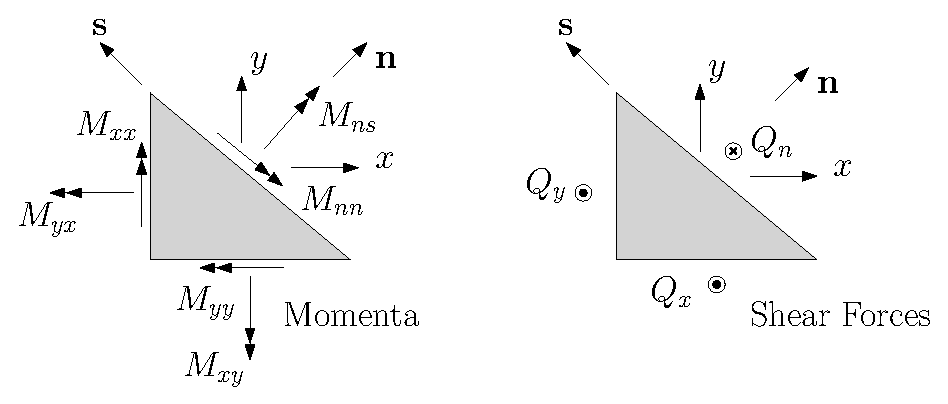
\includegraphics[width=0.7\textwidth]{Cauchy_law.eps}
\end{tcolorbox}
\end{frame}

\begin{frame}{Energy flow}
	Again the boundary values can be found by evaluating the time derivative of the Hamiltonian
	\footnotesize{
	\begin{equation*}
	\begin{aligned}
	\dot{H}&= \int_{\Omega} \left\{ \diffp{\alpha_w}{t} e_w  + \diffp{\bm\alpha_\theta}{t} \cdot \bm{e}_\theta + \diffp{\mathbb{A}_{\kappa}}{t} \cddot \mathbb{E}_{\kappa}  + \diffp{\bm\alpha_{\epsilon_s}}{t} \cdot \bm{e}_{\epsilon_s} \right\} \d\Omega \\
	&= \int_{\Omega} \left\{ \mathrm{div}(\bm{e}_{\epsilon_s}) e_w  + \left[\mathrm{Div}(\mathbb{E}_{\kappa}) + \bm{e}_{\epsilon_s} \right] \cdot \bm{e}_\theta + \mathrm{Grad}(\bm{e}_{\theta}) \cddot \mathbb{E}_{\kappa}  + (\mathrm{grad} (e_w) - \bm{e}_{\theta}) \cdot \bm{e}_{\epsilon_s} \right\} \d\Omega \\
	&= \int_{\partial \Omega} \left\{ \underbrace{(\bm{n} \cdot \bm{e}_{\epsilon_s})}_{Q_n} e_w  + (\bm{n} \cdot \mathbb{E}_{\kappa}) \cdot \bm{e}_\theta \right\} \d\Omega\,, \\
	&= \int_{\partial \Omega} \left\{ Q_n e_w  + (\bm{n} \cdot \mathbb{E}_{\kappa}) \cdot (\omega_n \bm{n} + \omega_s \bm{s}) \right\} \d\Omega\,, \\&= \int_{\partial \Omega} \left\{ Q_n e_w  + \omega_n  \underbrace{\bm{n}^T \mathbb{E}_{\kappa} \bm{n}}_{M_{nn}} + \omega_s \underbrace{\bm{s}^T \mathbb{E}_{\kappa} \bm{n}}_{M_{ns}} \right\} \d\Omega\,, \\
	&= \int_{\partial \Omega} \left\{ \blue{Q_n} \red{e_w}  + \blue{\omega_n} \red{M_{nn}} + \blue{\omega_s} \red{M_{ns}} \right\} \d\Omega\,.  \\
	\end{aligned}
	\end{equation*}
	}
\normalsize
Same result as in the vectorial case but with intrinsic operators.
\end{frame}

\subsection{Weak Formulation with different choices of boundary inputs}

\begin{frame}{Weak Formulation}
	The first line is multiplied  by $v_w$ (multiplication by a scalar) 
	\[\int_{\Omega} v_w \diffp{\alpha_w}{t}  \d\Omega =  \int_{\Omega} v_w \mathrm{div}(\bm{e}_{\epsilon_s}) \, \d\Omega,
	\]
	the second and the fourth lines by $\bm{v}_{\theta}$, $\bm{v}_{\epsilon_s}$ (scalar product of $\mathbb{R}^2$) 
	\begin{align*}
	\int_{\Omega} \bm{v}_{\theta} \cdot \diffp{\bm\alpha_{\theta}}{t}   \d\Omega &= \int_{\Omega} \bm{v}_{\theta} \cdot (\mathrm{Div}( \mathbb{E}_{\kappa}) + \bm{e}_{\epsilon_s}) \,  \d\Omega, \\
	\int_{\Omega} \bm{v}_{\epsilon_s} \cdot \diffp{\bm\alpha_{\epsilon_s}}{t}   \d\Omega &= \int_{\Omega} \bm{v}_{\epsilon_s} \cdot (\mathrm{grad}({e}_{w}) - \bm{e}_{\theta}) \, \d\Omega, 
	\end{align*}
	the third one by $\mathbb{V}_{\kappa}$ (tensor contraction)
	\[\int_{\Omega} \mathbb{V}_{\kappa} \cddot \diffp{\mathbb{A}_{\kappa}}{t}   \d\Omega = \int_{\Omega} \mathbb{V}_{\kappa} \cddot \mathrm{Grad}(\bm{e}_\theta) \, \d\Omega.
	\]
\end{frame}	

\begin{frame}{Choice I: Boundary control through forces and momenta}
The first two line of the system in weak form are integrated by parts
	\begin{equation*}
	\int_{\Omega} v_w \mathrm{div}(\bm{e}_{\epsilon_s})  \d\Omega = \int_{\partial \Omega} v_w \underbrace{\bm{n} \cdot \bm{e}_{\epsilon_s}}_{\blue{Q_n}}  \d s - \int_{\Omega} \mathrm{grad}(v_w)  \cdot \bm{e}_{\epsilon_s}  \d\Omega,
	\end{equation*}
	\small{
	\begin{equation*}
	\int_{\Omega} \bm{v}_{\theta} \cdot (\mathrm{Div}(\mathbb{E}_{\kappa}) + \bm{e}_{\epsilon_s})  \d\Omega = \int_{\partial \Omega} \bm{v}_{\theta} \cdot (\bm{n} \cdot \mathbb{E}_{\kappa})  \d s -\int_{\Omega} \left\{ \mathrm{Grad}(\bm{v}_{\theta}) \cddot \mathbb{E}_{\kappa} - \bm{v}_{\theta} \cdot \bm{e}_{\epsilon_s}\right\}  \d\Omega.
	\end{equation*}
	}
	\normalsize
	The usual additional manipulation is performed on the boundary term containing the momenta, so that the proper boundary values arise
	\begin{equation*}
	\begin{aligned}
	\int_{\partial \Omega} \bm{v}_{\theta} \cdot (\bm{n} \cdot \mathbb{E}_{\kappa})  \d s &= \int_{\partial \Omega} \left\{\underbrace{(\bm{v}_{\theta} \cdot \bm{n})}_{v_{\omega_n}} \bm{n} + \underbrace{(\bm{v}_{\theta} \cdot \bm{s})}_{v_{\omega_s}} \bm{s} \right\} \cdot (\bm{n} \cdot \mathbb{E}_{\kappa}) \,  \d s \\
	&= \int_{\partial \Omega} \left\{ v_{\omega_n} \blue{M_{nn}} + v_{\omega_s} \blue{M_{ns}} \right\}  \d s.
	\end{aligned}
	\end{equation*}

\end{frame}

\begin{frame}
The final system exhibits as \blue{control inputs} the boundary forces and momenta
\begin{exampleblock}{Weak Form with forces and momenta as inputs}
	\scriptsize
	\begin{equation*}
	\begin{cases}
	\displaystyle\int_{\Omega} v_w \diffp{\alpha_w}{t}  \d\Omega  &= - \displaystyle\int_{\Omega} \mathrm{grad}(v_w)  \cdot \bm{e}_{\epsilon_s}  \d\Omega +  \displaystyle\int_{\partial \Omega} v_w \blue{Q_n}  \d s \vspace{2mm}\\
	\displaystyle\int_{\Omega} \bm{v}_{\theta} \cdot \diffp{\bm\alpha_{\theta}}{t}   \d\Omega &=  -\displaystyle\int_{\Omega} \left\{ \mathrm{Grad}(\bm{v}_{\theta}) \cddot \mathbb{E}_{\kappa} - \bm{v}_{\theta} \cdot \bm{e}_{\epsilon_s}\right\}  \d\Omega + \displaystyle\int_{\partial \Omega} \left\{ v_{\omega_n} \blue{M_{nn}} + v_{\omega_s} \blue{M_{ns}} \right\}\d s \vspace{2mm} \\
	\displaystyle\int_{\Omega} \mathbb{V}_{\kappa} \cddot \diffp{\mathbb{A}_{\kappa}}{t}   \d\Omega &= \displaystyle\int_{\Omega} \mathbb{V}_{\kappa} \cddot \mathrm{Grad}(\bm{e}_\theta)  \d\Omega  \vspace{2mm} \\
	\displaystyle\int_{\Omega} \bm{v}_{\epsilon_s} \cdot \diffp{\bm\alpha_{\epsilon_s}}{t}   \d\Omega &= \displaystyle\int_{\Omega} \bm{v}_{\epsilon_s} \cdot (\mathrm{grad}({e}_{w}) - \bm{e}_{\theta})  \d\Omega
	\end{cases}.
	\end{equation*}
\end{exampleblock}

\normalsize{
	In this first case,  the boundary controls $\bm{u}_\partial$ and the corresponding output $\bm{y}_\partial$ are 
	\[\bm{u}_\partial = 
	\begin{pmatrix}
	\blue{{Q}_n } \\
	\blue{M_{nn}} \\
	\blue{M_{ns}} \\
	\end{pmatrix}_{\partial \Omega}, \qquad
	\bm{y}_\partial = 
	\begin{pmatrix}
	\red{e_w} \\
	\red{\omega_n} \\
	\red{\omega_s} \\
	\end{pmatrix}_{\partial \Omega}.
	\]
}
\end{frame}

\begin{frame}{Choice II: Boundary control through kinematic variables}
	If instead the last two lines are integrated by parts
	\begin{exampleblock}{Weak Form with linear and rotational velocities as inputs}
	\scriptsize
	\begin{equation*}
	\begin{cases}
	\displaystyle\int_{\Omega} v_w \diffp{\alpha_w}{t}  \d\Omega  &= \displaystyle \int_{\Omega} v_w \mathrm{div}(\bm{e}_{\epsilon_s})  \d\Omega \vspace{2mm}\\
	\displaystyle\int_{\Omega} \bm{v}_{\theta} \cdot \diffp{\bm\alpha_{\theta}}{t}   \d\Omega &= \displaystyle \int_{\Omega} \bm{v}_{\theta} \cdot (\mathrm{Div}(\mathbb{E}_{\kappa}) + \bm{e}_{\epsilon_s}) \;  \d\Omega \vspace{2mm} \\
	\displaystyle\int_{\Omega} \mathbb{V}_{\kappa} \cddot \diffp{\mathbb{A}_{\kappa}}{t}   \d\Omega &= - \displaystyle\int_{\Omega} \mathrm{Div}(\mathbb{V}_{\kappa}) \cdot \bm{e}_\theta \;  \d\Omega +  \displaystyle\int_{\partial \Omega} \left\{ v_{M_{nn}} \blue{\omega_{n}} + v_{M_{ns}} \blue{\omega_{s}} \right\}  \d s \vspace{2mm} \\
	\displaystyle\int_{\Omega} \bm{v}_{\epsilon_s} \cdot \diffp{\bm\alpha_{\epsilon_s}}{t}   \d\Omega &=  - \displaystyle\int_{\Omega} \left\{ \mathrm{div}(\bm{v}_{\epsilon_s}) e_w + \bm{v}_{\epsilon_s} \cdot \bm{e}_{\theta} \right\} \, \d\Omega + \displaystyle\int_{\partial \Omega} v_{Q_{n}} \blue{e_{w}} \;  \d s
	\end{cases}
	\end{equation*}
	\end{exampleblock}
	\normalsize
	where $v_{M_{nn}} = \bm{n}^T \mathbb{V}_{\kappa} \bm{n}, \;  v_{M_{ns}} = \bm{s}^T \mathbb{V}_{\kappa} \bm{n} \;$ and $v_{Q_n} = \bm{v}_{\epsilon_s} \cdot \bm{n}$.
	In this second case,  the boundary controls $\bm{u}_\partial$ and corresponding output $\bm{y}_\partial$ are
	\[\bm{u}_\partial = 
	\begin{pmatrix}
	\blue{e_w} \\
	\blue{\omega_{n}} \\
	\blue{\omega_{s}} \\
	\end{pmatrix}_{\partial \Omega}, \qquad
	\bm{y}_\partial = 
	\begin{pmatrix}
	\red{Q_n} \\
	\red{M_{nn}} \\
	\red{M_{ns}} \\
	\end{pmatrix}_{\partial \Omega}.
	\]
\end{frame}

\begin{frame}{Summary for the Mindlin Plate}
Main  points:
\begin{itemize}
\item variational derivative w.r.t. a tensor quantity;
\item strong tensorial form;
\item structure preserving weak formulation with different choices of the boundary inputs;
\item only two choices for the boundary inputs were shown but others are possible.
\end{itemize}
\end{frame}

\section{Vectorial PH formulation of the Kirchhoff plate} 

\begin{frame}{Energy and co-energy variables}
This model is the 2D extension of the Bernoulli beam. It is logical to select as energy variable the linear momentum, together with the curvatures

\begin{equation*}
\bm{\alpha} = (\mu v,\ \kappa_{xx},\ \kappa_{yy},\ \kappa_{xy})^T
\end{equation*}

where $v = \diffp{w}{t}$. The Hamiltonian density is given by 
\begin{equation*}
\mathcal{H} =\frac{1}{2} \bm{\alpha}^T \begin{bmatrix}
\frac{1}{\mu} & 0 \\
0 & \bm{D} \\
\end{bmatrix} \bm{\alpha}
\end{equation*}

So the variational derivative of the total Hamiltonian $H = \int_{\Omega} \mathcal{H} \ d\Omega$ provides as co-energy variables
\begin{equation*}
\mathbf{e} := \diffd{H}{\bm{\alpha}} = (v,\ M_{xx},\ M_{yy},\ M_{xy})^T
\end{equation*}
 
\end{frame}



\begin{frame}{Definition of J and boundary variables}
The skew-adjoint operator relating energies and co-energies is found to be 
\begin{equation*}
J = 
\begin{bmatrix}
0 & -\diffp[2]{}{x} & -\diffp[2]{}{y} & - \left(\diffp{}{y,x} + \diffp{}{x,y} \right)\\
\diffp[2]{}{x} & 0 & 0 & 0 \\
\diffp[2]{}{y} & 0 & 0 & 0 \\
\diffp{}{y,x} + \diffp{}{x,y} & 0 & 0 & 0 \\
\end{bmatrix}, 	\qquad
\diffp{\bm{\alpha}}{t} = J \mathbf{e}.
\end{equation*}
\begin{tcolorbox}
	From the Schwarz theorem for $C^2$ functions the mixed derivative could be be expressed as $2 \diffp{}{x,y}$, instead of $\diffp{}{y,x} + \diffp{}{x,y}$. However, in this way the symmetry intrinsically present in $\gamma_{xy} = -z \left( \diffp{w}{y,x} + \diffp{w}{x,y} \right)$ would be lost. The mixed derivative is here split to reestablish the symmetric nature of curvatures and momenta (that are of tensorial nature).
\end{tcolorbox}

\end{frame}

\section{Tensorial PH formulation of the Kirchhoff plate}

\begin{frame}{A scalar-tensor formulation}
The momenta and curvatures are of tensorial nature. In Cartesian coordinates
\begin{equation*}
\mathbb{K} = 
\begin{bmatrix}
\kappa_{xx} &  \kappa_{xy}\\
\kappa_{xy} & \kappa_{yy} \\
\end{bmatrix}, \qquad
\mathbb{M}=
\begin{bmatrix}
M_{xx} & M_{xy} \\
M_{xy} & M_{yy} \\
\end{bmatrix},
\end{equation*}
where now $\kappa_{xy}$ now is half the value of the one in the vectorial case. The curvatures tensor is the linear deformation tensor applied to the rotation vector $\bm{\theta} = \mathrm{grad}(w)$
\begin{equation*}
\mathbb{K} = \mathrm{Grad}(\bm{\theta}) =  \mathrm{Grad}(\mathrm{grad}(w)).
\end{equation*}
The momenta are found by introducing a fourth order tensor $\mathbb{D}$, such that $\mathbb{M}_{ij} = \mathbb{D}_{ijkl} \, \mathbb{K}_{kl}$
\end{frame}

\begin{frame}
For what concerns the choice of the energy variables a scalar and a tensor variable are grouped together
\begin{equation*}
\alpha_w = \mu \diffp{w}{t} \qquad \mathbb{A}_{\kappa} = \mathbb{K} 
\end{equation*}	
The Hamiltonian energy is written as
\begin{equation*}
H = \int_{\Omega} \left\{ \frac{1}{2} \mu \left(\diffp{w}{t} \right)^2 + \frac{1}{2} \mathbb{M} \cddot \mathbb{K}  \right\}  \d{\Omega} ,
\end{equation*}
The co-energy variables are found by computing the variational derivative of the Hamiltonian
\begin{equation*}
e_w := \diffd{H}{\alpha_w} = \diffp{w}{t},  \qquad  \mathbb{E}_{\kappa} := \diffd{H}{\mathbb{A}_{\kappa}} = \mathbb{M}.
\end{equation*}
\end{frame}

\subsection{Strong form}

\begin{frame}{Interconnection structure}
The formally skew-symmetric operator $J$ can be highlighted 
\begin{exampleblock}{Strong form for the Kirchhoff plate}
\begin{equation*}
\diffp{}{t}
\begin{pmatrix}
\alpha_w \\
\mathbb{A}_{\kappa} \\
\end{pmatrix} = 
\underbrace{\begin{bmatrix}
	0  &  -  \mathrm{div} \circ \mathrm{Div} \\
	\mathrm{Grad} \circ \mathrm{grad} & 0 \\
	\end{bmatrix}}_{J}
\begin{pmatrix}
e_w \\
\mathbb{E}_{\kappa} \\
\end{pmatrix}.
\end{equation*}
\end{exampleblock}

where all zeros are intended as nullifying operator from the space of input variables to the space of output variables.
\begin{theorem}[See \cite{BrugnoliKir} for additional details]
	The adjoint of $\mathrm{div} \circ \mathrm{Div}$ is $\mathrm{Grad} \circ \mathrm{grad}$ (i.e. the Hessian operator)
\end{theorem}

\begin{remark}
	The interconnection structure $J$ now resembles that of the Bernoulli beam. The double divergence and the double gradient coincide, in dimension one, with the second derivative.
\end{remark}
\end{frame}

\subsection{Weak Formulation with different choices of boundary inputs}

\begin{frame}{Weak Formulation}
The fist line  is multiplied  by $v_w$ (scalar multiplication)

\[
\int_{\Omega} v_w \diffp{\alpha_w}{t} \,  \d\Omega =  \int_{\Omega} -v_w \, \mathrm{div}(\mathrm{Div}(\mathbb{E}_{\kappa})) \, \d\Omega,
\]
the second line by $\mathbb{V}_{\kappa}$ (tensor contraction)
\[
\int_{\Omega} \mathbb{V}_{\kappa} \cddot \diffp{\mathbb{A}_{\kappa}}{t} \,  \d\Omega = \int_{\Omega} \mathbb{V}_{\kappa} \cddot  \mathrm{Grad}(\mathrm{grad}(e_w)) \,   \d\Omega.
\]
Now depending on which line is integrated by parts different boundary control term can be selected. 
\end{frame}

\begin{frame}{Choice I: Boundary control through forces and momenta}
The first line has to be integrated by parts \red{twice}
\small
\begin{equation*}
\int_{\Omega} - v_w \mathrm{div}(\mathrm{Div}(\mathbb{E}_{\kappa})) \, \d\Omega = \int_{\partial \Omega} \underbrace{- \bm{n} \cdot \mathrm{Div}(\mathbb{E}_{\kappa})}_{\blue{Q_n}} v_w \, \d{s} + \int_{\Omega} \mathrm{grad}(v_w)  \cdot \mathrm{Div}(\mathbb{E}_{\kappa}) \, \d\Omega
\end{equation*}
\normalsize
Applying again the integration by parts
\small
\begin{equation*}
\int_{\Omega} \mathrm{grad}(v_w)  \cdot \mathrm{Div}(\mathbb{E}_{\kappa}) \, \d\Omega = \int_{\partial \Omega} \mathrm{grad}(v_w)  \cdot \left( \bm{n} \cdot \mathbb{E}_{\kappa} \right) \, \d{s} -  \int_{\Omega}\mathrm{Grad}(\mathrm{grad}(v_w))  \cddot \mathbb{E}_{\kappa} \, \d\Omega
\end{equation*}
\normalsize
The usual additional manipulation is performed on the boundary terms, so that the proper boundary values arise
\small
\begin{equation*}
\begin{aligned}
\int_{\partial \Omega} \mathrm{grad}(v_w)  \cdot \left( \bm{n} \cdot \mathbb{E}_{\kappa} \right) \, \d{s} &= \int_{\partial \Omega} \left(\diffp{v_w}{n} \bm{n} + \diffp{v_w}{s} \bm{s} \right)  \cdot \left( \bm{n} \cdot \mathbb{E}_{\kappa} \right) \, \d{s} \\
&= \int_{\partial \Omega} \left\{  \diffp{v_w}{n}  \underbrace{\bm{n}^T \mathbb{E}_{\kappa}\bm{n}}_{\blue{M_{nn}}} +  \diffp{v_w}{s}  \underbrace{\bm{s}^T \mathbb{E}_{\kappa}\bm{n}}_{\blue{M_{ns}}} \right\}  \, \d{s} \\
&= \sum_{\Gamma_{i} \subset \partial \Omega} \left[ M_{ns} v_w \right]_{\partial \Gamma_i} + \int_{\partial \Omega} \left\{ \diffp{v_w}{n} \blue{M_{nn}}  - v_w  \diffp{\blue{M_{ns}}}{s} \right\} \d{s}
\end{aligned}
\end{equation*}
\end{frame}

\begin{frame}
Defining the effective shear stress as $\blue{\widetilde{Q}_n} = \blue{Q_n} - \diffp{\blue{M_{ns}}}{s}$ 
If the boundary is regular the final expression becomes
\small
\begin{equation*}
\int_{\Omega} v_w \diffp{\alpha_w}{t}  \, \d\Omega =  -  \int_{\Omega} \mathrm{Grad}(\mathrm{grad}(v_w))  \cddot \mathbb{E}_{\kappa} \, \d\Omega +  \int_{\partial \Omega} \left\{ \diffp{v_w}{n} \blue{M_{nn}}  + v_w \, \blue{\widetilde{Q}_n} \right\} \, \d{s}. 
\end{equation*}
\normalsize
\begin{exampleblock}{Weak form with forces and momenta as inputs}
	\footnotesize
	\begin{equation*}
	\begin{cases}
	\displaystyle\int_{\Omega} v_w \diffp{\alpha_w}{t} \, \d\Omega  &=  -  \displaystyle\int_{\Omega} \mathrm{Grad}(\mathrm{grad}(v_w))  \cddot \mathbb{E}_{\kappa} \, \d\Omega +  \displaystyle\int_{\partial \Omega} \left\{ \diffp{v_w}{n} \blue{M_{nn}}  + v_w \, \blue{\widetilde{Q}_n} \right\}   \, \d{s},  \vspace{2mm}\\
	\displaystyle\int_{\Omega} \mathbb{V}_{\kappa} \cddot \diffp{\mathbb{A}_{\kappa}}{t} \, \d\Omega &= \displaystyle\int_{\Omega} \mathbb{V}_{\kappa} \cddot \mathrm{Grad}(\mathrm{grad}(e_w)) \, \d\Omega. 
	\end{cases}
	\end{equation*}
\end{exampleblock}

\normalsize
The control input $\bm{u}_\partial$ and the corresponding conjugate outputs $\bm{y}_\partial$ are 
\[\bm{u}_\partial = 
\begin{pmatrix}
\blue{\widetilde{Q}_n} \\
\blue{M_{nn}} \\
\end{pmatrix}_{\partial \Omega}, \qquad
\bm{y}_\partial = 
\begin{pmatrix}
\red{e_w} \\
\displaystyle \red{\diffp{e_w}{n}} \\
\end{pmatrix}_{\partial \Omega}.
\]

\end{frame}

\begin{frame}{Choice II: Boundary control through kinematic variables}
	The same procedure can be performed on the second line of the system 
	\begin{exampleblock}{Weak form with linear and angular velocities as inputs}
	\small
	\begin{equation*}
	\begin{cases}
	\displaystyle\int_{\Omega} v_w \diffp{\alpha_w}{t} \d\Omega&=  \displaystyle\int_{\Omega} -v_w \, \mathrm{div}(\mathrm{Div}(\mathbb{E}_{\kappa}))  \d\Omega, \vspace{2mm}\\
	\displaystyle\int_{\Omega} \mathbb{V}_{\kappa} \cddot \diffp{\mathbb{A}_{\kappa}}{t}   \d\Omega&= \displaystyle\int_{\Omega} \mathrm{div}(\mathrm{Div}(\mathbb{V}_{\kappa})) e_w  d\Omega +  \displaystyle\int_{\partial \Omega} \left\{ {v}_{M_{nn}} \blue{\diffp{e_w}{n}}  + v_{\widetilde{Q}_n} \blue{e_w} \right\} \d{s}. 
	\end{cases}
	\end{equation*}
	\end{exampleblock}
	\normalsize
	where ${v}_{M_{nn}} = \bm{n}^T \mathbb{V}_{\kappa} \bm{n} \; $ and $ \; v_{\widetilde{Q}_n} = - \displaystyle \mathrm{Div}(\mathbb{V}_{\kappa}) \cdot \bm{n} - \diffp{ (\bm{s}^T \mathbb{V}_{\kappa} \bm{n}) }{s}.$ \\
	The control input $\bm{u}_\partial$ are now the kinematic boundary conditions, the corresponding conjugate outputs $\bm{y}_\partial$ are the dynamic boundary condition
	\[\bm{u}_\partial = 
	\begin{pmatrix}
	\blue{e_w} \\
	\displaystyle \blue{\diffp{e_w}{n}} \\
	\end{pmatrix}_{\partial \Omega}, \qquad
	\bm{y}_\partial = 
	\begin{pmatrix}
	\red{\widetilde{Q}_n} \\
	\red{M_{nn}} \\
	\end{pmatrix}_{\partial \Omega}.
	\]
\end{frame}

\begin{frame}{Summary for the Kirchhoff Plate}
Main  points:
\begin{itemize}
	\item new distributed port-Hamiltonian system involving second order differential operator in space dimension 2 for $J$;
	\item strong tensorial form where $\mathrm{div} \circ \mathrm{Div}=(\mathrm{Grad} \circ \mathrm{grad})^*$;
	\item structure preserving weak formulation with different choices of the boundary inputs;
	\item only two choices for the boundary variables were shown but others are possible;
\end{itemize} 
Other contribution (not presented here):
\begin{itemize}
	\item definition of the underlying Stokes-Dirac structure for the vectorial formulation of the Kirchhoff plate \cite{BrugnoliKir}.
\end{itemize}

\end{frame}




\section{Partition Finite Element method (PFEM) for Numerics}

\begin{frame}{Main Reference}
\nobibliography*

\bibentry{CardosoRibeiro2018}
\end{frame}


\begin{frame}{General principles of the structure preserving discretization}
	The energy, co-energy and test functions of the \textit{same} index are discretized by using the \textit{same} bases:
	\small
	\begin{equation*}
	\begin{aligned}
	\alpha_i^{ap} &:= \sum_{k=1}^{N_i} \phi_i^k(x,y) \alpha_i^k(t),  \\
	\alpha_i^{ap} &:= \bm{\phi}_i(x,y)^T \bm{\alpha}_i(t), \\
	\end{aligned} \qquad 
	\begin{aligned}
	e_i^{ap} &:= \sum_{k=1}^{N_i} \phi_i^k(x,y) e_i^k(t), \\
	e_i^{ap} &:= \bm{\phi}_i(x,y)^T \bm{e}_i(t), \\
	\end{aligned} \qquad 
	\begin{aligned}
	v_i^{ap} &:= \sum_{k=1}^{N_i} \phi_i^k(x,y) v_i^k,  \\
	v_i^{ap} &:= \bm{\phi}_i(x,y)^T \bm{v}_i. \\
	\end{aligned}
	\end{equation*}
	\normalsize
	The same procedure is applied for the boundary terms with a specific basis $\bm\psi$
	\begin{equation*}
	u_{\partial, i} \approx u_{\partial, i}^{ap} := \sum_{k=1}^{n_{\partial, i}} \psi^k_i(s) u_{\partial, i}^k(t) = \bm{\psi}_i(s)^T \bm{u}_{\partial, i}(t).
	\end{equation*}
	
	\begin{remark}
		The functions $\bm{\psi}_i(s)$ can be selected as the restriction of functions $\bm{\phi}$ over the boundary $\bm{\psi}(s) = \bm{\phi}(x(s),y(s))$ or in other ways.
	\end{remark}
	
\end{frame}


\subsection{Mindlin Plate}

\begin{comment}
	
\begin{frame}{Discretizing the vectorial weak form of Mindlin plate}
	Vectorial formulation in weak form with forces and momenta as input
	\scriptsize
	\begin{equation*}
	\underbrace{\int_{\Omega} \bm{\phi}_1 \bm{\phi}_1^T d\Omega}_{M_1} \; \dot{\bm{\alpha}}_1 = - \underbrace{\int_{\Omega}  \diffp{\bm{\phi}_1}{x} \bm{\phi}_7^T d\Omega}_{D_{x, 71}^T} \; \bm{e}_7 - \underbrace{\int_{\Omega}  \diffp{\bm{\phi}_1}{y} \bm{\phi}_8^T d\Omega}_{D_{y, 81}^T} \; \bm{e}_8 
	+\underbrace{\int_{\partial \Omega} \bm{\phi}_1 \bm{\psi}_1^T ds}_{B_{11}} \; \bm{u}_{\partial, 1},
	\end{equation*}	
	\begin{multline*}
	\underbrace{\int_{\Omega} \bm{\phi}_2 \bm{\phi}_2^T d\Omega}_{M_2}  \; \dot{\bm{\alpha}}_2 =  -\underbrace{\int_{\Omega}  \diffp{\bm{\phi}_2}{x} \bm{\phi}_4^T d\Omega}_{D_{x, 42}^T} \; \bm{e}_4 -\underbrace{\int_{\Omega}  \diffp{\bm{\phi}_2}{y} \bm{\phi}_6^T d\Omega}_{D_{y, 62}^T} \; \bm{e}_6 +  \underbrace{\int_{\Omega}  \bm{\phi}_2 \bm{\phi}_7^T d\Omega}_{D_{0, 27}} \; \bm{e}_7 \\
	+\underbrace{\int_{\partial \Omega} \bm{\phi}_2 \bm{\psi}_2^T n_x  ds}_{B_{22}} \; \bm{u}_{\partial, 2} \underbrace{-\int_{\partial \Omega} \bm{\phi}_2 \bm{\psi}_3^T n_y ds}_{B_{23}} \; \bm{u}_{\partial, 3},
	\end{multline*}	
	\begin{multline*}
	\underbrace{\int_{\Omega} \bm{\phi}_3 \bm{\phi}_3^T d\Omega}_{M_3} \; \dot{\bm{\alpha}}_3 =   -\underbrace{\int_{\Omega}  \diffp{\bm{\phi}_3}{y} \bm{\phi}_5^T d\Omega}_{D_{y, 53}^T} \; \bm{e}_5 -\underbrace{\int_{\Omega}  \diffp{\bm{\phi}_3}{x} \bm{\phi}_6^T d\Omega}_{D_{x, 63}^T} \; \bm{e}_6 + \underbrace{\int_{\Omega}  \bm{\phi}_3 \bm{\phi}_8^T d\Omega}_{D_{0, 38}} \; \bm{e}_8 \\
	+\underbrace{\int_{\partial \Omega} \bm{\phi}_3 \bm{\psi}_2^T n_y  ds}_{B_{32}} \; \bm{u}_{\partial, 2} + \underbrace{\int_{\partial \Omega} \bm{\phi}_3 \bm{\psi}_3^T n_x ds}_{B_{23}} \; \bm{u}_{\partial, 3},
	\end{multline*}

\end{frame}

\begin{frame}
Remaining lines of the system
\small
\begin{align*}
\underbrace{\int_{\Omega} \bm{\phi}_4 \bm{\phi}_4^T d\Omega}_{M_4}  \; \dot{\bm{\alpha}}_4 &=  \underbrace{\int_{\Omega} \bm{\phi}_4  \diffp{\bm{\phi}_2^T}{x}  d\Omega}_{D_{x, 42}} \; \bm{e}_2, \\
\underbrace{\int_{\Omega} \bm{\phi}_5 \bm{\phi}_5^T d\Omega}_{M_5}  \; \dot{\bm{\alpha}}_5 &=  \underbrace{\int_{\Omega} \bm{\phi}_5  \diffp{\bm{\phi}_3^T}{y}  d\Omega}_{D_{y, 53}} \; \bm{e}_3, \\
\underbrace{\int_{\Omega} \bm{\phi}_6 \bm{\phi}_6^T d\Omega}_{M_6} \; \dot{\bm{\alpha}}_6 &=  \underbrace{\int_{\Omega} \bm{\phi}_6  \diffp{\bm{\phi}_2^T}{y}  d\Omega}_{D_{y, 62}} \; \bm{e}_2 + \underbrace{\int_{\Omega} \bm{\phi}_6  \diffp{\bm{\phi}_3^T}{x}  d\Omega}_{D_{x, 63}} \; \bm{e}_3, \\
\underbrace{\int_{\Omega} \bm{\phi}_7 \bm{\phi}_7^T d\Omega}_{M_7}  \dot{\bm{\alpha}}_7 &=  \underbrace{\int_{\Omega} \bm{\phi}_7  \diffp{\bm{\phi}_1^T}{x}  d\Omega}_{D_{x, 71}} \; \bm{e}_1 - \underbrace{\int_{\Omega} \bm{\phi}_7  \bm{\phi}_2^T d\Omega}_{D_{0, 27}^T} \; \bm{e}_2, \\ 
\underbrace{\int_{\Omega} \bm{\phi}_8 \bm{\phi}_8^T d\Omega}_{M_8}  \dot{\bm{\alpha}}_8 &=  \underbrace{\int_{\Omega} \bm{\phi}_8  \diffp{\bm{\phi}_1^T}{y}  d\Omega}_{D_{y, 81}} \; \bm{e}_1 - \underbrace{\int_{\Omega} \bm{\phi}_8  \bm{\phi}_3^T d\Omega}_{D_{0, 38}^T} \; \bm{e}_3, 
\end{align*}

\end{frame}

\end{comment}

\begin{frame}{Mindlin Plate: discretized operators}
The formally skew-symmetric operator $J$ is replaced with the following skew-symmetric matrix
 \small
 \begin{equation*}
 J_d = 
 \begin{bmatrix}
 0 & 0 & 0 & 0 & 0 & 0 & -D_{x, 71}^T & -D_{y, 81}^T \\
 0 & 0 & 0 & -D_{x, 42}^T & 0 & -D_{y, 62}^T & D_{0, 27} & 0 \\
 0 & 0 & 0 & 0 & -D_{y, 53}^T & -D_{x, 63}^T & 0 & D_{0, 38} \\
 0 & D_{x, 42} & 0 & 0 & 0 & 0 & 0 & 0\\
 0 & 0 & D_{y, 53} & 0 & 0 & 0 & 0 & 0\\
 0 & D_{y, 62} & D_{x, 63} & 0 & 0 & 0 & 0 & 0\\
 D_{x, 71} & -D_{0, 27}^T & 0 & 0 & 0 & 0 & 0 & 0\\
 D_{y, 81} & 0 & -D_{0, 38}^T & 0 & 0 & 0 & 0 & 0\\
 \end{bmatrix}. 
 \end{equation*}
 As a consequence of the integration by parts, a control input is included in the finite-dimensional system. Matrix $B$ is defined by
 
 \begin{equation*}
 B = 
 \begin{bmatrix}
 B_{11} & 0 & 0 \\
 0 & B_{22} & B_{23} \\
 0 & B_{32} & B_{33} \\
 0_{\nu_4 \times n_{\partial, 1}} & 0_{ \nu_4 \times n_{\partial, 2}} & 0_{\nu_4 \times n_{\partial, 3}} \\
 \end{bmatrix}.
 \end{equation*}
\end{frame}

\begin{frame}{Final discretized system}
The final system is written as
\begin{equation*}
\begin{aligned}
M \dot{\bm{\alpha}} &= J_d  \,\bm{e} + B \, \bm{u}_{\partial}, \\
\bm{y}_{\partial} &= B^T \bm{e}
\end{aligned}   
\end{equation*}
where
\begin{itemize}
\item $M = \text{Diag}[M_1,M_2,M_3,M_4,M_5,M_6,M_7,M_8]$ is a block diagonal matrix, \\
\item $\bm{\alpha}$ is simply the concatenation of the $\bm\alpha_i$ (just like $\bm{e}$) \\
\item $\bm{u}_{\partial}$ is the concatenation of the $\bm{u}_{\partial, i}$ ($\bm{u}_{\partial, 1}= Q_n, \bm{u}_{\partial, 2}= M_{nn}$ and $\bm{u}_{\partial, 3}= M_{ns}$). 
\end{itemize}
   
\end{frame}

\subsection{Kirchhoff Plate}

\begin{comment}
	
\begin{frame}{Discretizing the vectorial weak form of Kirchhoff plate}
Vectorial formulation in weak form with forces and momenta as input
\scriptsize
\begin{multline*}
\underbrace{\int_{\Omega} \bm{\phi}_1 \bm{\phi}_1^T \, \d\Omega}_{M_1} \; \dot{\bm{\alpha}}_1 = - \underbrace{\int_{\Omega}  \diffp[2]{\bm{\phi}_1}{x} \bm{\phi}_2^T \, \d\Omega}_{D_{xx}^T} \; \bm{e}_2 - \underbrace{\int_{\Omega}  \diffp[2]{\bm{\phi}_1}{y} \bm{\phi}_3^T \, \d\Omega}_{D_{yy}^T} \; \bm{e}_3 - 2 \underbrace{\int_{\Omega} \diffp{\bm{\phi}_1}{x,y} \bm{\phi}_4^T \, \d\Omega}_{D_{xy}^T} \; \bm{e}_4\\
+\underbrace{\int_{\partial \Omega} \bm{\phi}_1 \bm{\psi}_1^T \, \d{s}}_{B_1} \; \bm{u}_{\partial, 1} + \underbrace{\int_{\partial \Omega} \diffp{\bm{\phi}_1}{n} \bm{\psi}_2^T \, \d{s}}_{B_2} \; \bm{u}_{\partial, 2},
\end{multline*}

\begin{align*}
\underbrace{\int_{\Omega} \bm{\phi}_2 \bm{\phi}_2^T \, \d\Omega}_{M_2}  \; \dot{\bm{\alpha}}_2 =  \underbrace{\int_{\Omega} \bm{\phi}_2  \diffp[2]{\bm{\phi}_1^T}{x} \, \d\Omega}_{D_{xx}} \; \bm{e}_1, \\
\underbrace{\int_{\Omega} \bm{\phi}_3 \bm{\phi}_3^T \, \d\Omega}_{M_3}  \; \dot{\bm{\alpha}}_3 =  \underbrace{\int_{\Omega} \bm{\phi}_3  \diffp[2]{\bm{\phi}_1^T}{y} \, \d\Omega}_{D_{yy}} \; \bm{e}_1, \\
\underbrace{\int_{\Omega} \bm{\phi}_4 \bm{\phi}_4^T \, \d\Omega}_{M_4}  \; \dot{\bm{\alpha}}_4 = 2  \underbrace{\int_{\Omega} \bm{\phi}_4  \diffp{\bm{\phi}_1^T}{x,y} \, \d\Omega}_{D_{xy}} \; \bm{e}_1.  
\end{align*}

\end{frame}

\end{comment}

\begin{frame}{Kirchhoff Plate: discretized operators}
The discretized system is written as 
\begin{equation*}
\begin{pmatrix}
M_1 \dot{\bm{\alpha}}_1 \\
M_2 \dot{\bm{\alpha}}_2 \\
M_3 \dot{\bm{\alpha}}_3 \\
M_4 \dot{\bm{\alpha}}_4 \\
\end{pmatrix} =
\begin{bmatrix}
0   & -D_{xx}^T   & -D_{yy}^T   & -2 D_{xy}^T\\
D_{xx}   & 0   & 0   & 0\\
D_{yy}   & 0   & 0   & 0\\
2 D_{xy}   & 0   & 0   & 0 \\
\end{bmatrix}
\begin{pmatrix}
\bm{e}_1 \\
\bm{e}_2 \\
\bm{e}_3 \\
\bm{e}_4 \\
\end{pmatrix}+  
\begin{bmatrix}
B_1 & B_2\\
0   & 0\\
0   & 0\\
0   & 0 \\
\end{bmatrix}
\begin{pmatrix}
\bm{u}_{\partial, 1} \\
\bm{u}_{\partial, 2} \\
\end{pmatrix},
\end{equation*}
where $M_i$ are square matrices (of size $N_i\times N_i$), $D_{xx}$ is an $N_2 \times N_1$
matrix, $D_{yy}$ is an $N_3 \times N_1$ matrix, $D_{xy}$ is an $N_4 \times N_1$ matrix,  $B_1$ is an $N_1 \times N_{\partial, 1}$ matrix and finally $B_2$ is an $N_2 \times N_{\partial, 2}$ matrix.
The collocated output are defined as
\begin{equation*}
\bm{y}_{\partial} =
\begin{bmatrix}
B_1^T  & 0 & 0 & 0\\
B_2^T  & 0 & 0 & 0\\
\end{bmatrix}
\begin{pmatrix}
\bm{e}_1 \\
\bm{e}_2 \\
\bm{e}_3 \\
\bm{e}_4 \\
\end{pmatrix}.
\end{equation*}
\end{frame}

\section{General PFEM Variational Formulation and Numerical Results}

\begin{frame}{Variational formulation using PFEM}
The general variational form can be now stated:
\begin{itemize}
	\item Energy variables belong to the mixed space $\alpha \in  V_{\alpha} = V_{\alpha_1} \times  \dots \times V_{\alpha_n}$, where $\alpha_i \in V_{\alpha_i}$;
	\item  Coenergy variables $e = \mathcal{Q} \alpha$ where $\mathcal{Q}$ is a coercive symmetrical operator $\mathcal{Q}: V_{\alpha} \rightarrow V_{\alpha}$;
	\item Test functions belong to the same space as $\alpha$ $v \in V_{\alpha}$
\end{itemize}

\begin{block}{General structure preserving weak form with known inputs}
If the boundary input ${u}_\partial$ is known (i.e for the Mindlin plate free or clamped conditions) then
\begin{equation*}
m\left(v, \diffp{\alpha}{t}\right) = j(v,e) + b_{u_\partial}(v_{y_\partial}) \qquad \forall v \in V
\end{equation*}
where $m$ is the mass bilinear, symmetric and coercive form, $j$ is the interconnection bilinear and antisymmetric form and $b$ is a linear functional.
\end{block}


\end{frame}


\begin{frame}{Dealing with algebraic constraints}
If the boundary input vector is partly unknown then Lagrange multipliers and corresponding test function have to be introduced. Variables $\lambda_{u_\partial}, v_{u_\partial} \in V_{\lambda}$ defined over $\Gamma_{\lambda}$, the boundary subset where the input are unknown and the conjugated output are set to zero (e.g. clamped plate with a free side).
\begin{block}{General structure preserving weak form with unknown inputs}
\begin{equation*}
\begin{cases}
m\left(v, \diffp{\alpha}{t}\right) = j(v,e) + b(v_{y_\partial}, \lambda_{u_\partial}) \\
0 = c(v_{u_\partial}, e_{y_\partial})
\end{cases} \qquad \forall v \in V, \; \forall v_{u_\partial} \in V_\lambda
\end{equation*} 
where $v_{y_\partial} = \mathcal{B}_{y_\partial} v$ and $e_{y_\partial} = \mathcal{B}_{y_\partial} e$ ($\mathcal{B}$ is the boundary variables operator). Now $b$ is a bilinear form on spaces $V_{\alpha} \times V_{\lambda}$ and $c$ is defined over $V_{\lambda} \times V_{\alpha}$ and is obtained from $b$ by swapping variables and applying $\mathcal{B}_{y_\partial}$ on $e$ instead of $v$.
\end{block}
\end{frame} 


\begin{frame}{Numerical Study of the Mindlin Plate}
This PH system can be discretized using a FE software. These numerical results were obtained using Fenics.
To compare the eigenvalues publications 
\cite{duran1999approximation,dawe1980rayleigh,huang1984nine} were used : 

\footnotesize
\bibentry{duran1999approximation} \\
\bibentry{dawe1980rayleigh}\\
\bibentry{huang1984nine}

\normalsize
In the next tables these references will be denoted respectively by D-H, D-R, H-H. Our results are denoted by B-A.
\end{frame}

\begin{frame}{Study case}
	Properties of the plate
	\begin{itemize}
		\item Square plate with $l_x=l_y=1$;
		\item Young modulus $E = 70 \, GPa$;
		\item Density $\rho = 2000 \, kg/m^3$;
		\item Poisson modulus $\nu = 0.3$. 
	\end{itemize}
	Boundary conditions considered
	\begin{itemize}
		\item All clamped CCCC ($w = 0, \, \omega_s = 0, \, \omega_n = 0$); 
		\item Simply supported hard SSSS ($w = 0, \, \omega_s = 0$);
		\item Half clamped half simply supported SCSC;
		\item All clamped but one side free CCCF (F stands for free, i.e. $M_{nn} = 0, \ M_{ns} = 0, \ Q_{n} = 0,  $). 
	\end{itemize}


\end{frame}

\begin{frame}{Computational Complexity}
	A scalar viable discretized using $n$  $P^1$ elements for each side gives rise to $(n+1)\times(n+1)$ dofs and one discretized using $n$ $P^2$ elements contains $(2n+1)\times(2n+1)$ dofs. Hence since the system is of dimension 8:
	\begin{itemize}
		\item if 10 $P^1$ elements are used for each side the final system contains 968 states;
		\item if 10 $P^2$ elements are used for each side the final system contains 3528 states.
	\end{itemize}

\end{frame}

\begin{frame}{Benchmark variables}
	The variables are discretized by using Lagrange polynomials of order 1 (same order for each variable) or 2. Normalized eigenfrequency found in \cite{dawe1980rayleigh}  are used as benchmark 
	\[\widehat{\omega}_{mn} = \omega_{mn}^h L\left(\frac{2(1 + \nu)\rho}{E}\right)^{\frac{1}{2}} \quad \text{Final result independent on $E, \rho$},
	\]
	$m$ and $n$ being the numbers of half-waves occurring in the modes shapes in the $x$
	and $y$ directions, respectively. \\
	Colors used for comparing of the first 4 eigenvalues 
	\begin{itemize}
		\item \fcolorbox{black}{Blue}{\rule{0pt}{6pt}\rule{6pt}{0pt}} benchmark results;
		\item \fcolorbox{black}{Green}{\rule{0pt}{6pt}\rule{6pt}{0pt}} 1\% error or less;
		\item \fcolorbox{black}{Yellow}{\rule{0pt}{6pt}\rule{6pt}{0pt}} up to 5\% error;		
		\item \fcolorbox{black}{Orange}{\rule{0pt}{6pt}\rule{6pt}{0pt}} up to 15\% error;	
		\item \fcolorbox{black}{Red}{\rule{0pt}{6pt}\rule{6pt}{0pt}} spurious eigenvalue;	
	\end{itemize} 
	
	
	
\end{frame}


\begin{frame}{Eigenvalues for $t/L = 0.1$ using $P^1$}
\footnotesize
\begin{table}[h]
\centering
	\begin{tabular}{|c||c||m|c|g|c||c||o|}
	\hline 
	BCs					  & Mode &\tiny{$N:10$(B-A)}&\tiny{$N:10$(D-H)}&\tiny{$N:20$(B-A)} &\tiny{$N:20$(D-H)} & H-H & D-R \\ 
	\hline 
	\multirow{4}{*}{CCCC} &$\widehat{\omega}_{11}$& 1.5999& 1.5947& 1.5917& 1.5921& 1.591& 1.594\\
						  &$\widehat{\omega}_{21}$& 3.0615& 3.1181& 3.0410& 3.0595& 3.039& 3.046\\
	                      &$\widehat{\omega}_{12}$& 3.0615& 3.1181& 3.0410& 3.0595& 3.039& 3.046\\
	                      &$\widehat{\omega}_{22}$& 4.3161& 4.4477& 4.2682& 4.3106& 4.263& 4.285\\
	\hline	
	\multirow{4}{*}{SSSS} &$\widehat{\omega}_{11}$& 0.9324& 0.9384& 0.9324& 0.9323& 0.930& 0.930\\
						  &$\widehat{\omega}_{21}$& 2.2227& 2.2893& 2.2226& 2.2366& 2.219& 2.219\\
						  &$\widehat{\omega}_{12}$& 2.2227& 2.2893& 2.2226& 2.2366& 2.219& 2.219\\
						  &$\widehat{\omega}_{22}$& 3.4142& 3.5657& 3.3608& 3.4450& 3.405& 3.406\\
	\hline		
	\multirow{4}{*}{SCSC} &$\widehat{\omega}_{11}$& 1.3111& 1.3060& 1.3013& 1.3016& 1.300& 1.302\\
					   	  &$\widehat{\omega}_{21}$& 2.4155& 2.4664& 2.3966& 2.4120& 2.394& 2.398\\
						  &$\widehat{\omega}_{12}$& 2.9082& 2.9617& 2.8871& 2.9043& 2.885& 2.888\\
						  &$\widehat{\omega}_{22}$& 3.8906& 4.0126& 3.8458& 3.8830& 3.839& 3.852\\
	\hline
	\multirow{5}{*}{CCCF} &$\widehat{\omega}_{\frac{1}{2}1}$& 1.0855& 1.0812& 1.0982&	1.0848&	1.081&	1.089\\
						  &$\widehat{\omega}_{\frac{3}{2}1}$& 1.7636& 1.7759& 1.7461&	1.7525&	1.744&	1.758\\
						  &$\widehat{\omega}_{\frac{1}{2}2}$& 2.6696& 2.7413& 2.6575&	2.6787&	2.657&	2.673\\
						  &$\widehat{\omega}_{\frac{5}{2}1}$& 3.2248& 3.3186& 3.1997&	3.2282&	3.197&	3.216\\
	\hline 
	\end{tabular} 
\end{table}
\end{frame}

\begin{frame}{Eigenvalues for $t/L = 0.01$  using $P^1$}
\footnotesize
\begin{table}[h]
	\centering
	\begin{tabular}{|c||c||b|c|m|c||c||o|}
		\hline 
		BCs					  & Mode &\tiny{$N:10$(B-A)}&\tiny{$N:10$(D-H)}&\tiny{$N:20$(B-A)} &\tiny{$N:20$(D-H)} & H-H & D-R \\ 
		\hline 
		\multirow{4}{*}{CCCC} &$\widehat{\omega}_{11}$&	0.1967&	.1754&	.1765&	.1754&	.1754&	.1754\\
							  &$\widehat{\omega}_{21}$&	0.4030&	.3668&	.3604&	.3599&	.3574&	.3576\\
							  &$\widehat{\omega}_{12}$&	0.4030&	.3668&	.3604&	.3599&	.3574&	.3576\\
							  &$\widehat{\omega}_{22}$&	0.6431&	.5487&	.5358&	.5323&	.5264&	.5274\\
		\hline 	
		\multirow{4}{*}{SSSS} &$\widehat{\omega}_{11}$&	0.1706&	.0972&	.1128&	.0965&	.0963&	.0963\\
							  &$\widehat{\omega}_{21}$&	0.3576&	.2486&	.2660&	.2426&	.2406&	.2406\\
							  &$\widehat{\omega}_{12}$&	0.3576&	.2486&	.2660&	.2426&	.2406&	.2406\\
							  &$\widehat{\omega}_{22}$&	0.5803&	.4035&	.3865&	.3893&	.3847&	.3848\\
		\hline 			
		\multirow{4}{*}{SCSC} &$\widehat{\omega}_{11}$&	0.1864&	.1417&	.1487&	.1413&	.1411&	.1411\\
							  &$\widehat{\omega}_{21}$&	0.3649&	.2748&	.2829&	.2688&	.2668&	.2668\\
							  &$\widehat{\omega}_{12}$&	0.3987&	.3474&	.3485&	.3402&	.3377&	.3377\\
							  &$\widehat{\omega}_{22}$&	0.6075&	.4814&	.4933&	.4657&	.4604&	.4608\\
		\hline 		
		\multirow{5}{*}{CCCF} &$\widehat{\omega}_{\frac{1}{2}1}$& 0.1238& .1182& .1166& .1170&	.1166&	.1171\\
							  &$\widehat{\omega}_{\frac{3}{2}1}$& 0.2207& .1977& .1954& .1956&	.1949&	.1951\\
							  &$\widehat{\omega}_{\frac{1}{2}2}$& 0.3204& .3193& .3078& .3109&	.3080&	.3093\\
							  &$\widehat{\omega}_{\frac{5}{2}1}$& 0.4144& .3874& .3751& .3771&	.3736&	.3740\\			
		\hline 
	\end{tabular} 
\end{table}
\end{frame}


\begin{frame}{Eigenvalues for $t/L = 0.1$  using $P^2$}
\small
\begin{table}[h]
	\centering
	\begin{tabular}{|c||c||m|g||c||o|}
		\hline 
		BCs					  & Mode & $N=5$ (B-A) & $N=10$ (B-A) & H-H & D-R \\ 
		\hline
		\multirow{4}{*}{CCCC} &$\widehat{\omega}_{11}$& 1.5976&	1.5914&	1.591&	1.594\\ 
						      &$\widehat{\omega}_{21}$& 3.0584&	3.0405&	3.039&	3.046\\ 
		                      &$\widehat{\omega}_{12}$& 3.0677&	3.0405& 3.039&	3.046\\ 
		                      &$\widehat{\omega}_{22}$& 4.3109&	4.2662&	4.263&	4.285\\ 
		\hline 		
		\multirow{4}{*}{SSSS} &$\widehat{\omega}_{11}$& 0.9304&	0.9302&	0.930&	0.930\\ 
							  &$\widehat{\omega}_{21}$& 2.2223&	2.2194&	2.219&	2.219\\ 
		                      &$\widehat{\omega}_{12}$&	2.2224&	2.2194& 2.219&	2.219\\ 
							  &$\widehat{\omega}_{22}$& 3.4128&	3.4061&	3.405&	3.406\\		
		\hline 
		\multirow{4}{*}{SCSC} &$\widehat{\omega}_{11}$& 1.3053&	1.3004&	1.300&	1.302\\
							  &$\widehat{\omega}_{21}$& 2.4040&	2.3946&	2.394&	2.398\\
							  &$\widehat{\omega}_{12}$& 2.9060& 2.8858&	2.885&	2.888\\
							  &$\widehat{\omega}_{22}$& 3.8721&	3.8415&	3.839&	3.852\\
		\hline 		
		\multirow{4}{*}{CCCF} &$\widehat{\omega}_{\frac{1}{2}1}$& 1.0845& 1.0797& 1.081& 1.089\\
							  &$\widehat{\omega}_{\frac{3}{2}1}$& 1.7559& 1.7425& 1.744& 1.758\\	
							  &$\widehat{\omega}_{\frac{1}{2}2}$& 2.6762& 2.6547& 2.657& 2.673\\
							  &$\widehat{\omega}_{\frac{5}{2}1}$& 3.2186& 3.1954& 3.197& 3.216\\		
		\hline 
	\end{tabular} 
\end{table}
\end{frame}

\begin{frame}{Eigenvalues for $t/L = 0.01$  using $P^2$}
\small
\begin{table}[h]
	\centering
	\begin{tabular}{|c||c||m|g||c||o|}
		\hline 
		BCs					  & Mode & $N=5$ (B-A) & $N=10$ (B-A) & H-H & D-R \\ 
		\hline
		\multirow{4}{*}{CCCC} &$\widehat{\omega}_{11}$& 0.1872&	0.1762&	0.1754&	0.1754\\ 
							  &$\widehat{\omega}_{21}$& 0.3725&	0.3598&	0.3574&	0.3576\\ 
							  &$\widehat{\omega}_{12}$& 0.4055&	0.3598&	0.3574&	0.3576\\ 
							  &$\widehat{\omega}_{22}$& 0.6043&	0.5335&	0.5264&	0.5274\\ 	
		\hline 		
		\multirow{4}{*}{SSSS} &$\widehat{\omega}_{11}$& 0.0963&	0.0963&	0.0963&	0.0963\\ 
							  &$\widehat{\omega}_{21}$& 0.2422&	0.2406&	0.2406&	0.2406\\ 
							  &$\widehat{\omega}_{12}$& 0.2430&	0.2406&	0.2406&	0.2406\\ 
							  &$\widehat{\omega}_{22}$& 0.3874&	0.3848&	0.3847&	0.3848\\ 		
		\hline 
		\multirow{4}{*}{SCSC} &$\widehat{\omega}_{11}$& 0.1492&	0.1418&	0.1411&	0.1411\\ 
							  &$\widehat{\omega}_{21}$& 0.2827&	0.2683&	0.2668&	0.2668\\ 
							  &$\widehat{\omega}_{12}$& 0.3608&	0.3394&	0.3377&	0.3377\\ 
							  &$\widehat{\omega}_{22}$& 0.4940&	0.4654&	0.4604&	0.4608\\ 
		\hline 		
		\multirow{4}{*}{CCCF} &$\widehat{\omega}_{\frac{1}{2}1}$& 0.1197& 0.1169& 0.1166& 0.1171\\ 
							  &$\widehat{\omega}_{\frac{3}{2}1}$& 0.2092& 0.1960& 0.1949& 0.1951\\ 	
							  &$\widehat{\omega}_{\frac{1}{2}2}$& 0.3188& 0.3089& 0.3080& 0.3093\\ 
							  &$\widehat{\omega}_{\frac{5}{2}1}$& 0.3938& 0.3757& 0.3736& 0.3740\\ 
		\hline 
	\end{tabular} 
\end{table}
\end{frame}

\begin{frame}{Temporal Simulation}
Consider a uniform specific load acting on a clamped plate at rest
\begin{equation*}
\bm{f}(t) = 
\begin{cases}
-1  \; m/s^2 \, \hat{\bm{z}} \quad &t < 0.01 \ s \\
0 			\quad &t > 0.01 \ s\\
\end{cases}
\end{equation*}
Corresponding linear form: $l(v) = \int \rho h v_w f \d{\Omega}$. \\
Parameters:
\begin{itemize}
\item Total simulation time: $ T = 0.05$
\item Time step: $dt= 6.85 \, 10^{-6} s $ 
\item Integration in time: Stormer-Verlet
\end{itemize}

\end{frame}

\begin{frame}
\centering
\textbf{Simulation output $e_w = \diffp{w}{t}$ \\ (scale factor $\times 500$, 100 frame per second)}

\vspace{0.5cm}

\includemovie[poster, mouse=true, controls=true, toolbar=true, autostop=true]{10cm}{6cm}{./Animations/Loaded_Plate_Video.mp4} 
%\movie[start=0.0s, label=cells, height = 6cm, width=8cm, showcontrols=true, poster]{}{Video} 


\end{frame}

\begin{frame}
\centering
\includegraphics[width=0.8\textwidth]{Ham_MinLoaded.eps}
\end{frame}

\begin{frame}[allowframebreaks]
\bibliographystyle{unsrt}
\nocite{*}
\bibliography{bibliography_pres2}


\end{frame}

\begin{frame}
\centering
Thank you for your attention. Questions?
\end{frame}
\end{document}
